\section{Carrier Type by Hot Probe}

With usage of the hot probe it is found that voltage increases in the negative direction, indicating that the wafer is a p-type material. This is due to the majority carriers being holes.

\section{Resistivity by Four-Point Probe}

Based off of the topology of the sample under study we learn that the resistivity is given by the formula, with a depth (d) known as 300 $\mu m$:

\begin{equation}
    \rho = 4.53 \frac{V}{I} d
    \label{eqn:resist}
\end{equation}

A common atom which is used to dope silicon is the boron atom. This is possibly what the wafer was doped with. It is not possible with our suite of measurements to determine the exact doping material. Hoever we do know that the impuritiy concentration is approximately 3.9 $\e{14}cm^{-3}$ 

\begin{table}[H]
    \centering
    \begin{tabular}{@{}llll@{}}
\toprule
\textbf{V (Volts)} & \textbf{I (Amps)} & \textbf{\begin{tabular}[c]{@{}l@{}}Resistivity \\ ($\Omega \cdot cm$)\end{tabular}} & \textbf{\begin{tabular}[c]{@{}l@{}}Impurity \\ Concentration ($cm^{-3}$)\end{tabular}} \\ \midrule
0.0239             & $2.43\e{-4}$       & 13.4                                                                                & $3.9\e{14}$                                                                              \\ \bottomrule
\end{tabular}
    \caption{Values taken from 4 point measurement. Resistivity calculated using equation \ref{eqn:resist}, and impurity calculated using Figure \ref{fig:impurities}}
    \label{tab:4point}
\end{table}

\begin{figure}[H]
    \centering
    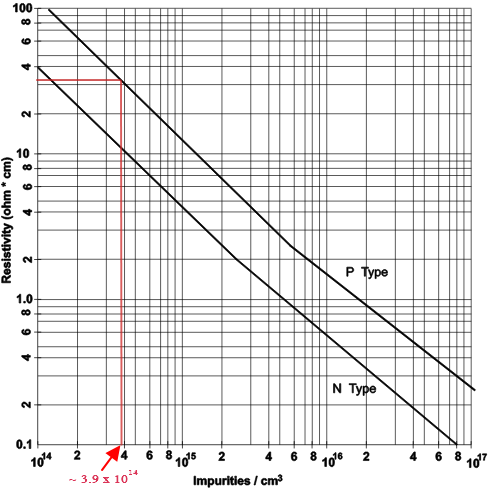
\includegraphics[width=.475\textwidth]{figures/Impurities.png}
    \caption{Resistivity verses impurity concentration in silicon. The calculated value for resistivity is matched with the level of impurities here.}
    \label{fig:impurities}
\end{figure}

\clearpage

\section{Sheet Resistance}

We now wish to investigate doped areas of the wafer to determine their resistance, specifically a quantity known as 
R$_\square$.

\begin{figure}[H]
    \centering
    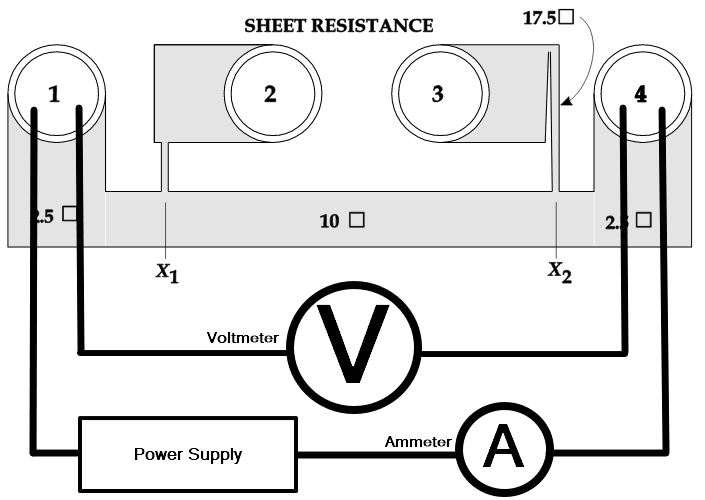
\includegraphics[width=.6\textwidth]{figures/circuit_diagram.png}
    \caption{Basic circuit diagram showing how resistance and current are measured in this probing method.}
    \label{fig:circuit}
\end{figure}

\begin{table}[H]
    \centering
    \begin{tabular}{@{}llll@{}}
\toprule
\textbf{V$_{1,4}$ (Volts)} & \textbf{I$_{1,4}$ (Amps)} & \textbf{R$_{1,4} $($\Omega $)} & \textbf{R$_\square$($\Omega / \square $)} \\ \midrule
3.529                      & $1.284\e{-3}$             & 2738                           & 182.33                                    \\ \bottomrule
\end{tabular}
    \caption{Values taken from sheet resistance measurement using points 1 and 4.}
    \label{tab:sheet_1}
\end{table}

After measuring this resistance directly between two pads (1,4), we use pads 1,4 as current pads and pads 2,3 as voltage pads, since the power is being supplied across 1,4 we can see that this is creating the voltage difference between pads 2 and 3. From this we are able to measure resistance and find R$_\square$ again based off of square value of 10. This is shown in Table \ref{tab:sheet_2}. From this we see that the value is smaller than that originally seen in the direct measurement. The difference which is found between the direct and indirect measurements is found to be significant as it is approximately 12\% of the overall signal. The effect of contact resistance from the probes is most likely the major factor which differentiates the R$_\square$ values.

\begin{table}[H]
    \centering
    \begin{tabular}{@{}llll@{}}
\toprule
\textbf{V$_{2,3}$ (Volts)} & \textbf{I$_{1,4}$ (Amps)} & \textbf{R$_{x1,x2} $($\Omega $)} & \textbf{R$_\square$($\Omega / \square $)} \\ \midrule
2.338                      & $1.39\e{-3}$              & 1682                             & 168.2                                     \\ \bottomrule
\end{tabular}
    \caption{Values taken from sheet resistance measurement using points 1 and 4 as current pads and 2,3 as voltage pads.}
    \label{tab:sheet_2}
\end{table}

\section{Measurement of the Finished Diode}
\begin{figure}[H]
    \centering
    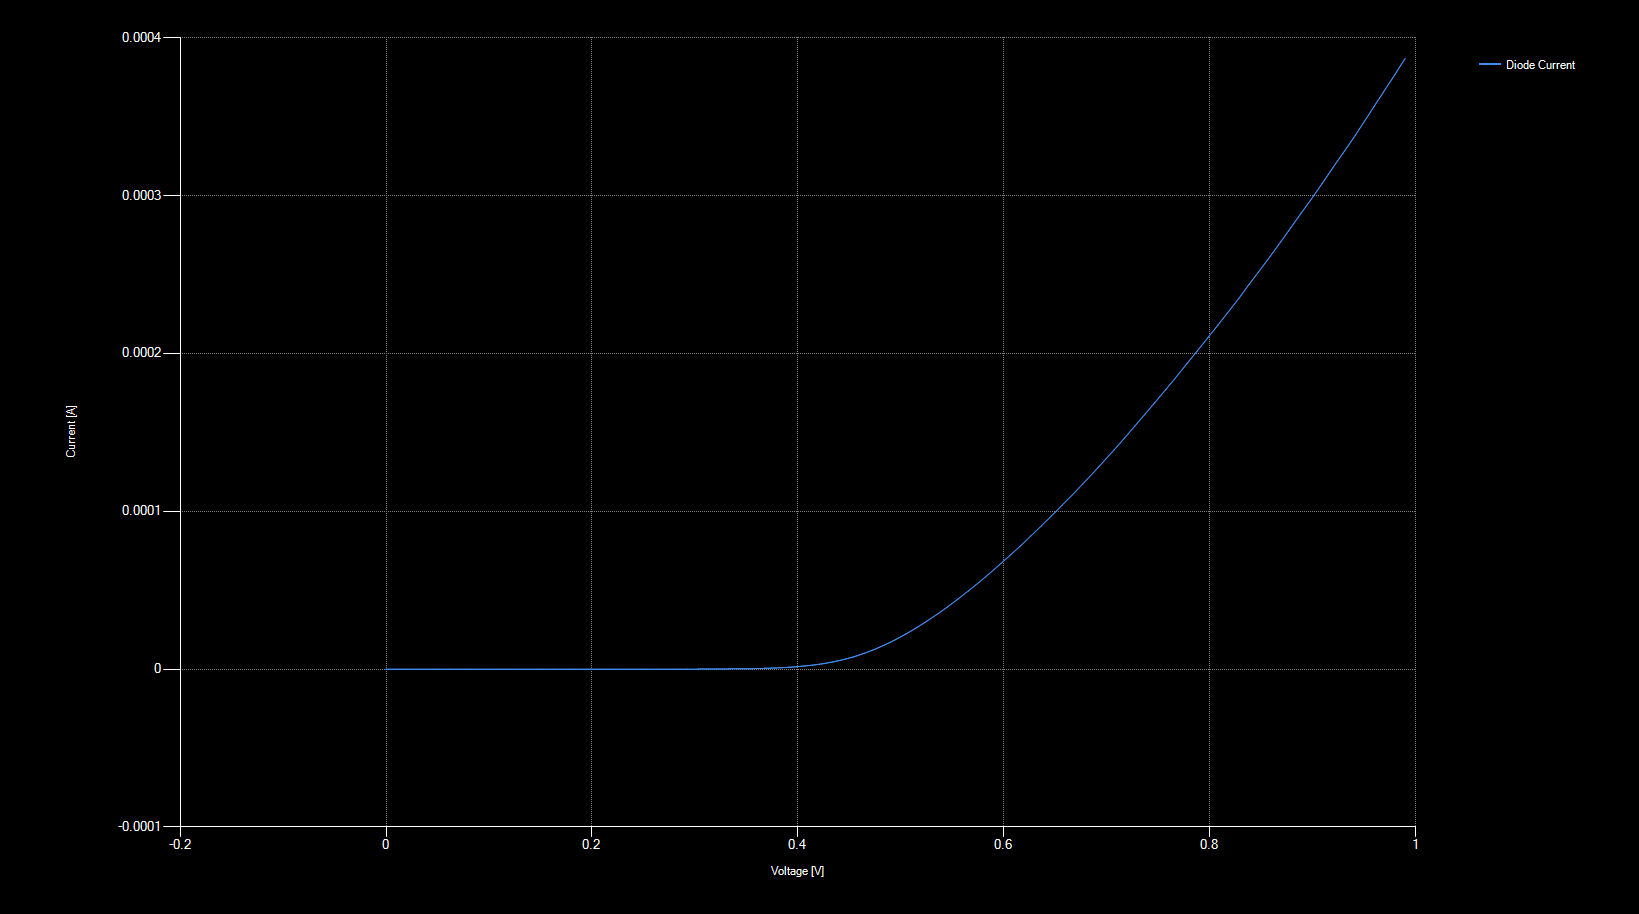
\includegraphics[width=.6\textwidth]{figures/Forward_Graph.png}
    \caption{Forward plot obtained in lab}
    \label{fig:forward}
\end{figure}
\begin{figure}[H]
    \centering
    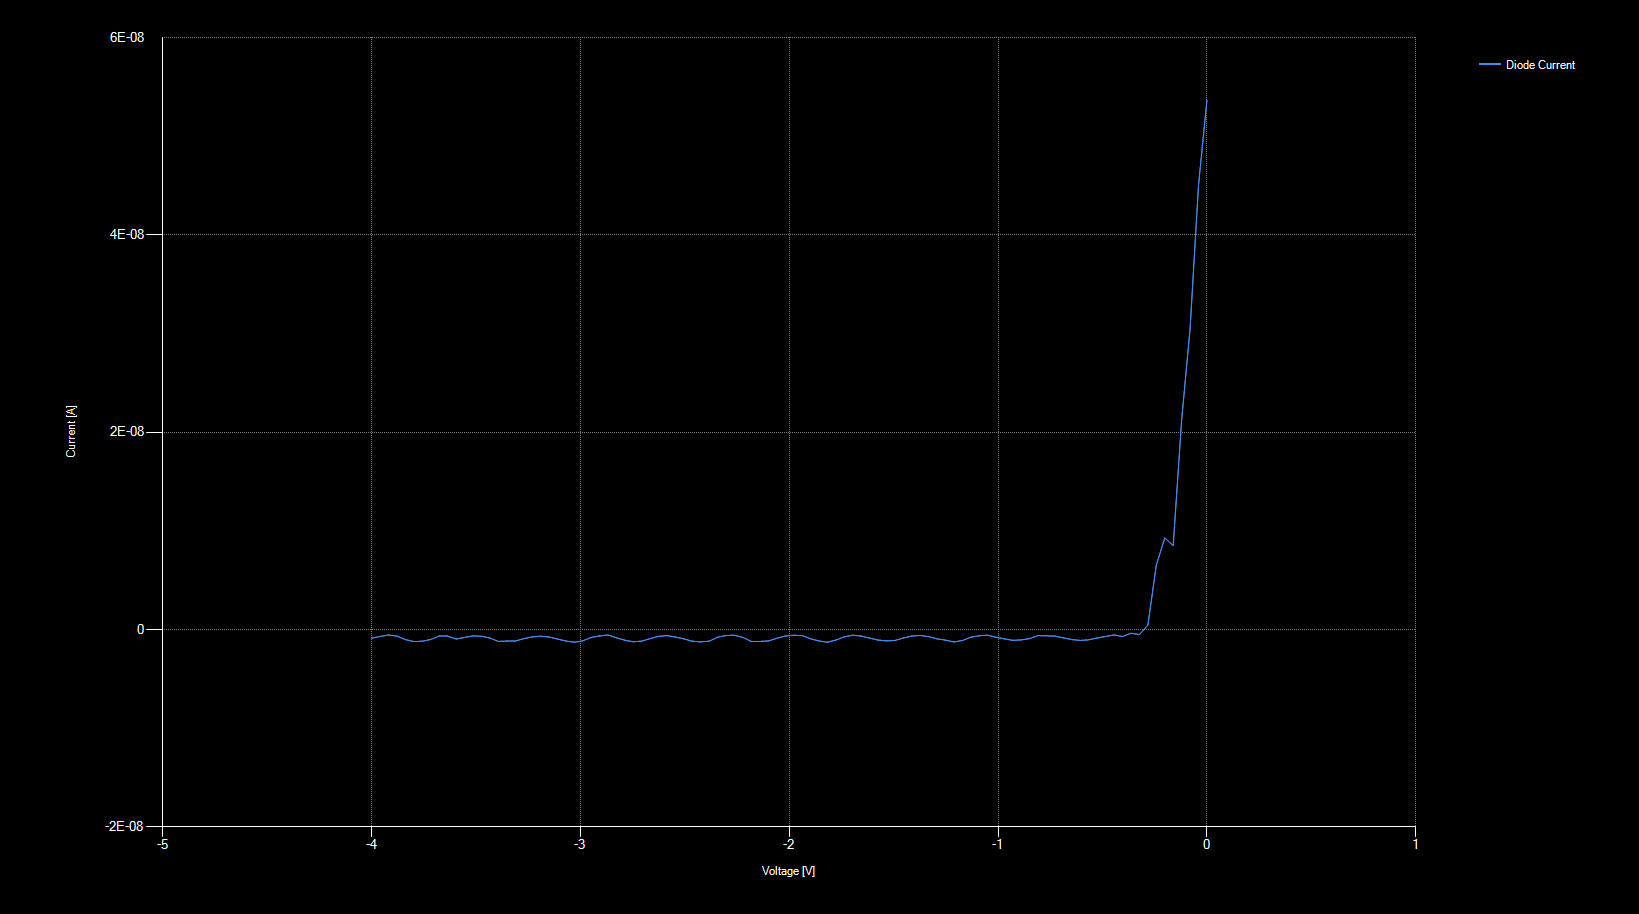
\includegraphics[width=.6\textwidth]{figures/Reverse_nolight.png}
    \caption{reverse plot obtained in lab. This one was done with no light}
    \label{fig:revnolight}
\end{figure}
\begin{figure}[H]
    \centering
    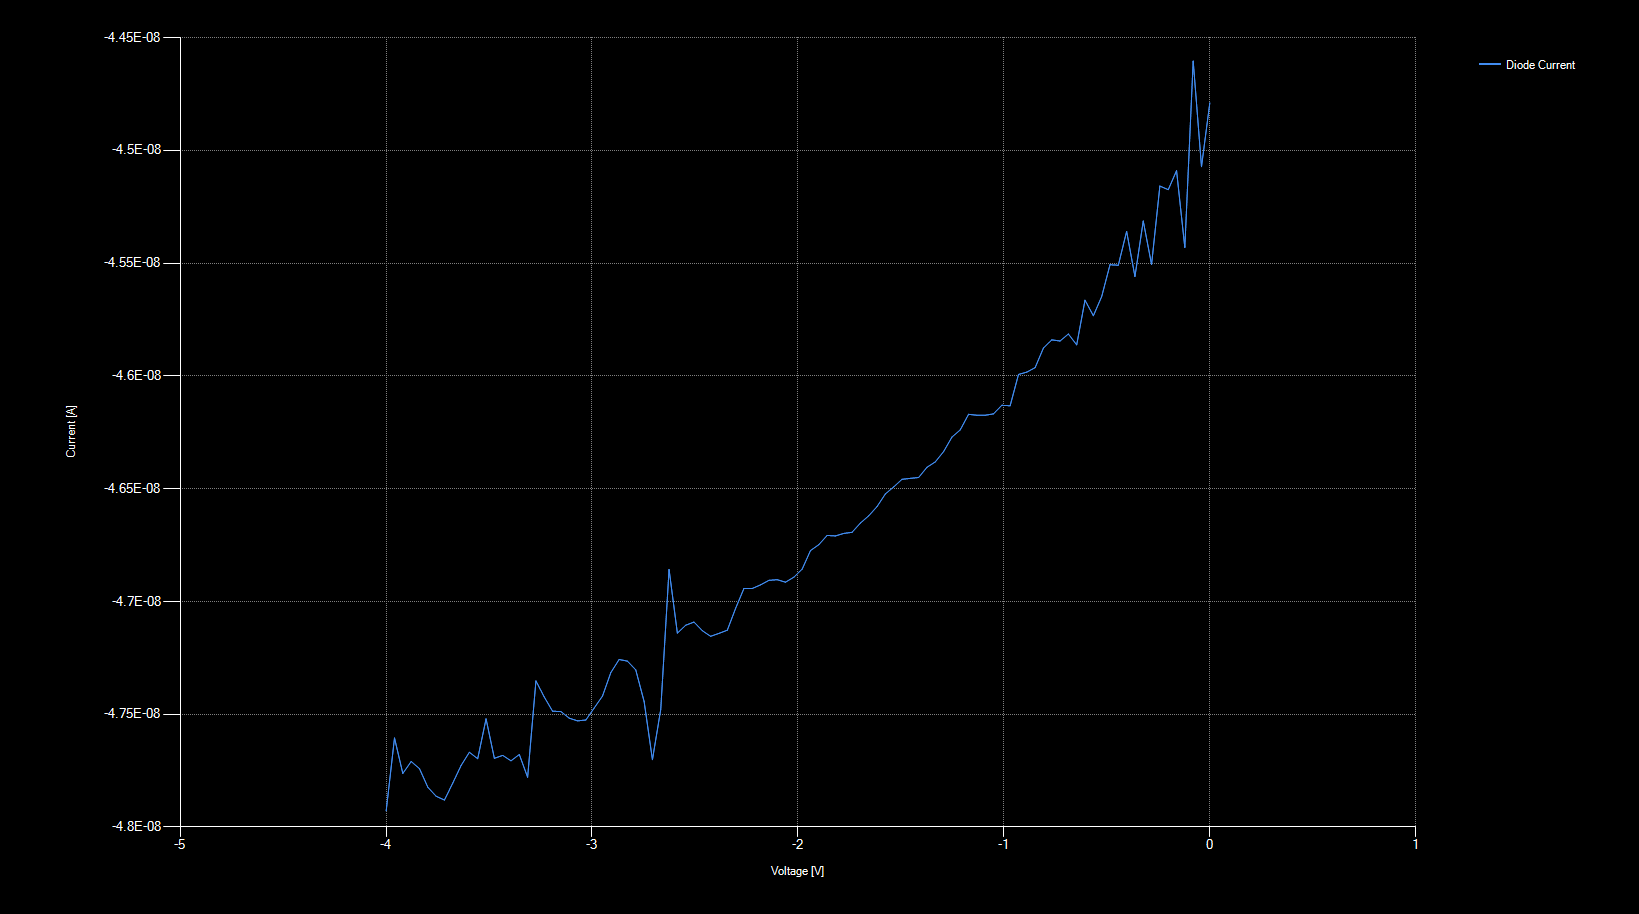
\includegraphics[width=.6\textwidth]{figures/Reverse_midlight.png}
    \caption{Reverse plot obtained in lab. This was done with mid light}
    \label{fig:revmidlight}
\end{figure}
\begin{figure}[H]
    \centering
    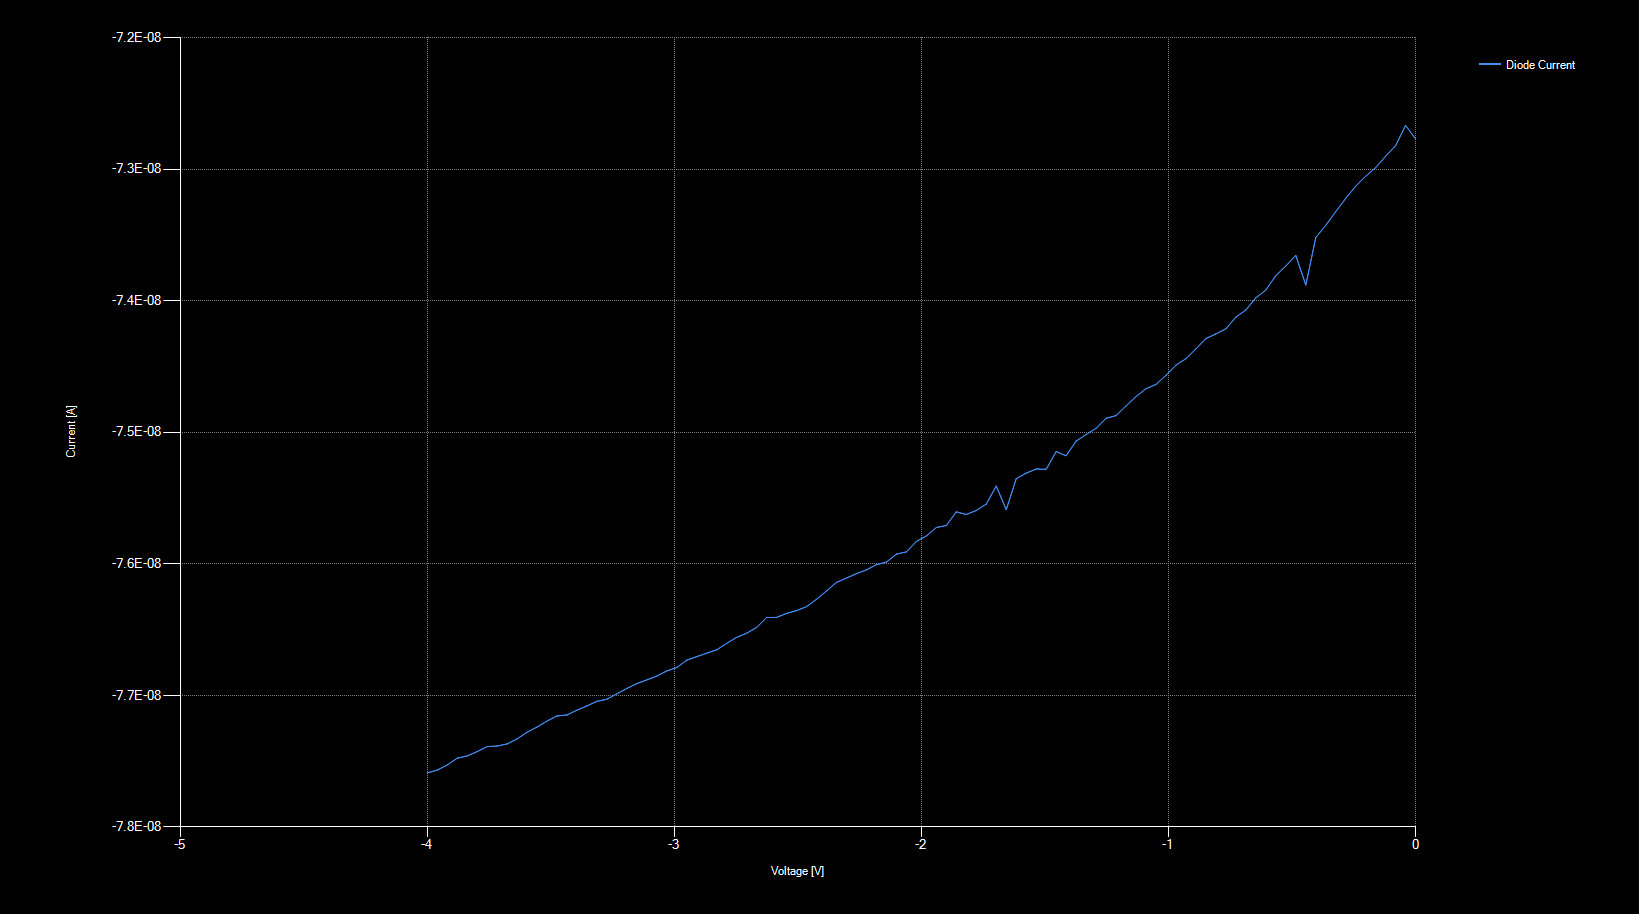
\includegraphics[width=.6\textwidth]{figures/reverse_highlight.png}
    \caption{Reverse plot obtained in lab done with high intensity light}
    \label{fig:revhighlight}
\end{figure}

\begin{figure}[H]
    \centering
    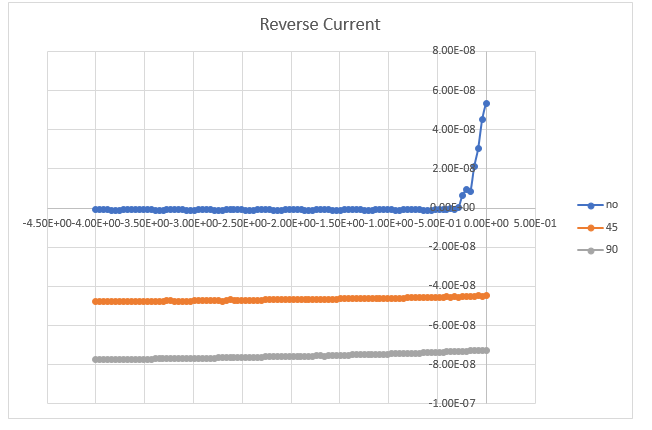
\includegraphics[width=.6\textwidth]{figures/Revese_current_sktech.png}
    \caption{sketch from the data taken}
    \label{fig:revhighlight}
\end{figure}



\section{Switching Diode}
\begin{table}[H]
    \centering
    \begin{tabular}{@{}llllll@{}}
\toprule
\textbf{V$_f$ (V)} & \textbf{V$_r$ (V)} & \textbf{t$_f $(microseconds)} & \textbf{t$_s$(microseconds)} & \textbf{|$V_s/V_f$|} & \textbf{$\tau_{po}$} \\ \midrule
5 &	-5 &	50	& 2.22	& 1	& 3.202782991\\
9 &	-1 &	50 &	8.95 &	9 &	3.886935613\\
3 &	-7 &	50 &	0.47 &	0.42 &	1.340341622\\
5 &	-5 &	5 &	1.06 &	1	
                                   \\ \bottomrule
\end{tabular}
    \caption{Values taken from the oscilloscope.}
    \label{tab:switching}
\end{table}

b)	In case one we see that the ratio between $V_f$ and $V_r$ is 1 and in case three that ratio is 0.42. We see that the tr value is much lower in case 3 compared to case 1. This means that the lower the ratio between the forward voltage and the reverse voltage the lower the shortage time. This is expected because  as we get from the lb manual When the generator switches from $V_f$ to $-V_r$, the carriers have to be evacuated before the diode is reverse biased and until the carriers are all pulled back, they will carry the forced reverse current -$V_r$/R in the diode, and this occurs for the storage time $t_s$. So when the ratio of $V_f$ to $V_r$ is lower it means that there are less carriers to evacuate leading to a shorter storage time\\
c)The calculates tau values are similar for two of the cases, those being case 1 and 2 while for case 3 it differs from the rest. I would estimate that the value of tau would be and average of these three values which is 2.81.\\
d)The reason we see a discrepancy between case one and case 4, namely case 4 having a much lower ts than case one has to do with the period. In case 1 the period is 100 microseconds making the half period 50 microseconds while in case 4 the half period is 10 microseconds. If you look at equation 4 you will find that the last case does not satisfy the equation at all. This again has to do with the fact that you have such a short period it does not allow for the carriers to be evacuated before the next period.\\

\section{Conclusion}\\
In this lab we looked at the properties of a silicon wafer and determined if it was a p-type or an n-type wafer based on the hot probe test. found the Impurity concentration by doing a four point probe and from that we found the resistivity. Next we determined the sheet resistance and finally we looked into the properties of diodes. Measuring a Finished diode under different light sources and the looking into the switching time of a diode. 